\section{Bancos de dados colunares} 
\label{sec:colunar}

A ideia por traz dos bancos de dados colunares não é nova. Uma das primeiras propostas de organizar os 
dados de um banco de dados por colunas, em vez da tradicional representação por linhas dos bancos de 
dados relacionais, apareceu em 1969 \citep{estabrook1969theory}. De forma resumida, enquanto um banco de 
dados relacional tradicional armazena cada registro ou tupla em um espaço contínuo do disco (ou memória), 
os bancos de dados colunares armazenam cada coluna em espaços contínuos \citep{Abadi2009}. 

A grande vantagem da representação colunar é a compressão de dados, uma vez que o domínio dos dados 
é preservado em espaços contíguos de disco ou memória. 
Uma das principais formas de compressão de dados é por dicionário, onde cada coluna de uma 
tabela (ou relação) é dividia em um índice com os valores distintos ordenados e um vetor com a 
codificação dos valores de cada tupla na mesma sequência em que aparecem na tabela. 
Esta codificação utiliza um numero mínimo de bits do domínio de valores de cada registro, 
baseada no dicionário. Com os dados comprimidos, menos Bytes trafegam entre o disco e a 
memória principal, tornando operações de consulta e agregação mais rápidas.
A Figura \ref{fig:tabular} mostra a representação tradicional de uma tabela num banco de dados 
relacional tradicional (orientado por linhas) e a Figura \ref{fig:colunar} mostra como a 
primeira coluna da relação é organizada em um banco de dados colunar com compressão por dicionário.

\begin{figure}[!htbp]
	\centering
	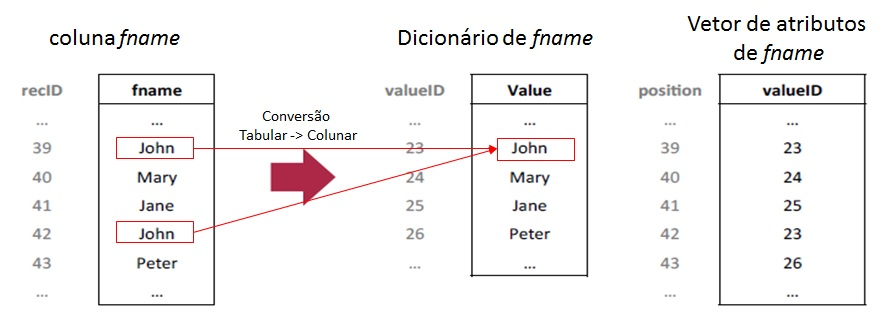
\includegraphics[width=\linewidth]{./Representacao_colunar.jpg}
	\caption{Organização da coluna fname em um banco de dados colunar.}
	\label{fig:colunar}
\end{figure}


Para explicar melhor o mecanismo de compressão, imaginemos que a coluna \textbf{fname} tenha 
100 caracteres representados por 1 Byte cada. Imaginemos também que a tabela em questão trata-se 
da lista de todos os cidadãos brasileiros, ou seja, teremos aproximadamente 200 milhões de registros. 
Logo, o espaço de armazenamento no modelo tradicional é de $200*10^6 * 100~Bytes \cong 18,62~GBytes$. 
No armazenamento em formato de colunas, os dados são armazenados em um dicionário que contém uma 
entrada para cada valor distinto. Imaginemos que há 10 mil nomes (primeiro nome) distintos no Brasil. 
Com isso, para o dicionário, precisamos de $10*10^3 * 100~Bytes \cong 1~MByte$. Já o vetor de 
valores conterá os 200 milhões de registros, mas codificados pela quantidade mínima de bits 
necessários para se codificar os 10 mil valores distintos $log_2 10.000 \cong 13,2$, ou seja, 
14 bits. Nesse caso, o vetor de valores terá $200*10^6 * 14~bits \cong 2,6~GBytes$. Nesse exemplo simples 
podemos observar um fator de compressão de $18,62 / (0,001 + 2,6) \cong 7,2$ vezes.

A recuperação de um determinado registro (tupla) passa por um acesso direto à posição dele em 
cada uma dos vetores de valor das colunas da tabela e mais um acesso em cada dicionário para traduzir 
a codificação no valor original.

O grande problema nessa representação são operações de remoção e inserção, que usualmente causam uma 
reorganização do dicionário e consequentemente uma reorganização de todos os dados das colunas cujo 
dicionário foi reordenado. Por isso, o uso desse tipo de tecnologia deve ser preferível em conjuntos 
de dados cuja operação predominante seja de consulta. Plattner \citep{plattner2009common} alega que 
os bancos de dados corporativos possuem uma carga predominantemente de consulta e com isso, 
pode-se unificar os repositórios OLTP e OLAP na mesma estrutura, sugerindo para tal, a representação colunar. 

Os sistemas modernos que utilizam a representação colunar lançam mão de diversas estratégias para 
minimizar esses efeitos de reorganização dos dicionários. O SAP HANA, por exemplo, divide os dados 
em principal e diferencial \citep{plattner2012memory}. Novos registros e atualizações de valores são 
incluídos no conjunto diferencial, que é mantido em tamanho pequeno. As operações de consulta juntam 
os dados do conjunto principal com o conjunto diferencial. Embora a busca no conjunto diferencial seja 
ineficiente, ela é realizada sobre um conjunto pequeno de dados. De tempos em tempos, os conjuntos são 
mesclados resultando em um novo conjunto principal e um conjunto diferencial praticamente vazio, que 
conterá apenas as operações realizadas durante a operação de mesclagem. 

Há também outros mecanismos de compressão para outros domínios de dados, e.g. números inteiros e de ponto 
flutuante \citep{Abadi2006, Zukowski2006}. É importante ressaltar que todos estes mecanismos de 
compressão de dados tentam balancear a taxa de compressão de dados com o processamento para compressão
e descompressão; em geral, os mecanismos mais eficientes em termos de taxa de compressão não são utilizados,
uma vez que o processamento (CPU) para descompressão dos dados durante a execução das consultas
pode ser um fator determinante. Adicionalmente, em geral, todos os mecanismos de compressão de dados
preservam as propriedades de igualdade e ordenação dos dados, i.e. valores $=$, $<$ ou $>$ no domínio original
dos dados são também $=$, $<$ ou $>$ no domínio de compressão. Esta propriedade é extremamente importante, 
pois a execução de diversos algoritmos da álgebra relacional que envolvem a comparação e ordenação dos
dados, e.g. junção, podem ser executados no domínio dos dados comprimidos, evitando assim processamento 
desnecessário de descompressão dos dados. É fácil observar esta propriedade no exemplo acima da compressão
da coluna \emph{fname}, desde que o dicionário esteja ordenado por nome.

Atualmente, os principais fornecedores de bancos de dados relacionais tradicionais também fornecem 
soluções de armazenamento colunar, como Microsoft, Oracle, IBM, SAP e outros. Entretanto, há sistemas
gerenciadores de bancos de dados puramente colunar, os comerciais SAP IQ e Actian Vectorwise, e os
de código aberto C-Store e MonetDB.
  

